\textcolor{black}{\section{Procedimiento}}

\subsection{PARTE 1}
El arreglo para poder observar el efecto Ramsauer-Townsend se muestra en la figura \cite{DiagT}. Primero usamos la bomba mecánica para extraer el aire dentro de la cámara de Townsend (Townsend's chamber), y después encendemos la bomba turbomolecular, hasta hacer un vacío de $200 Torr$. Después encendemos el láser EKSPLA NT 342B, tras verificar su funcionamiento, lo disparamos hacia el cátodo.

\begin{figure}[H]
	\centering
	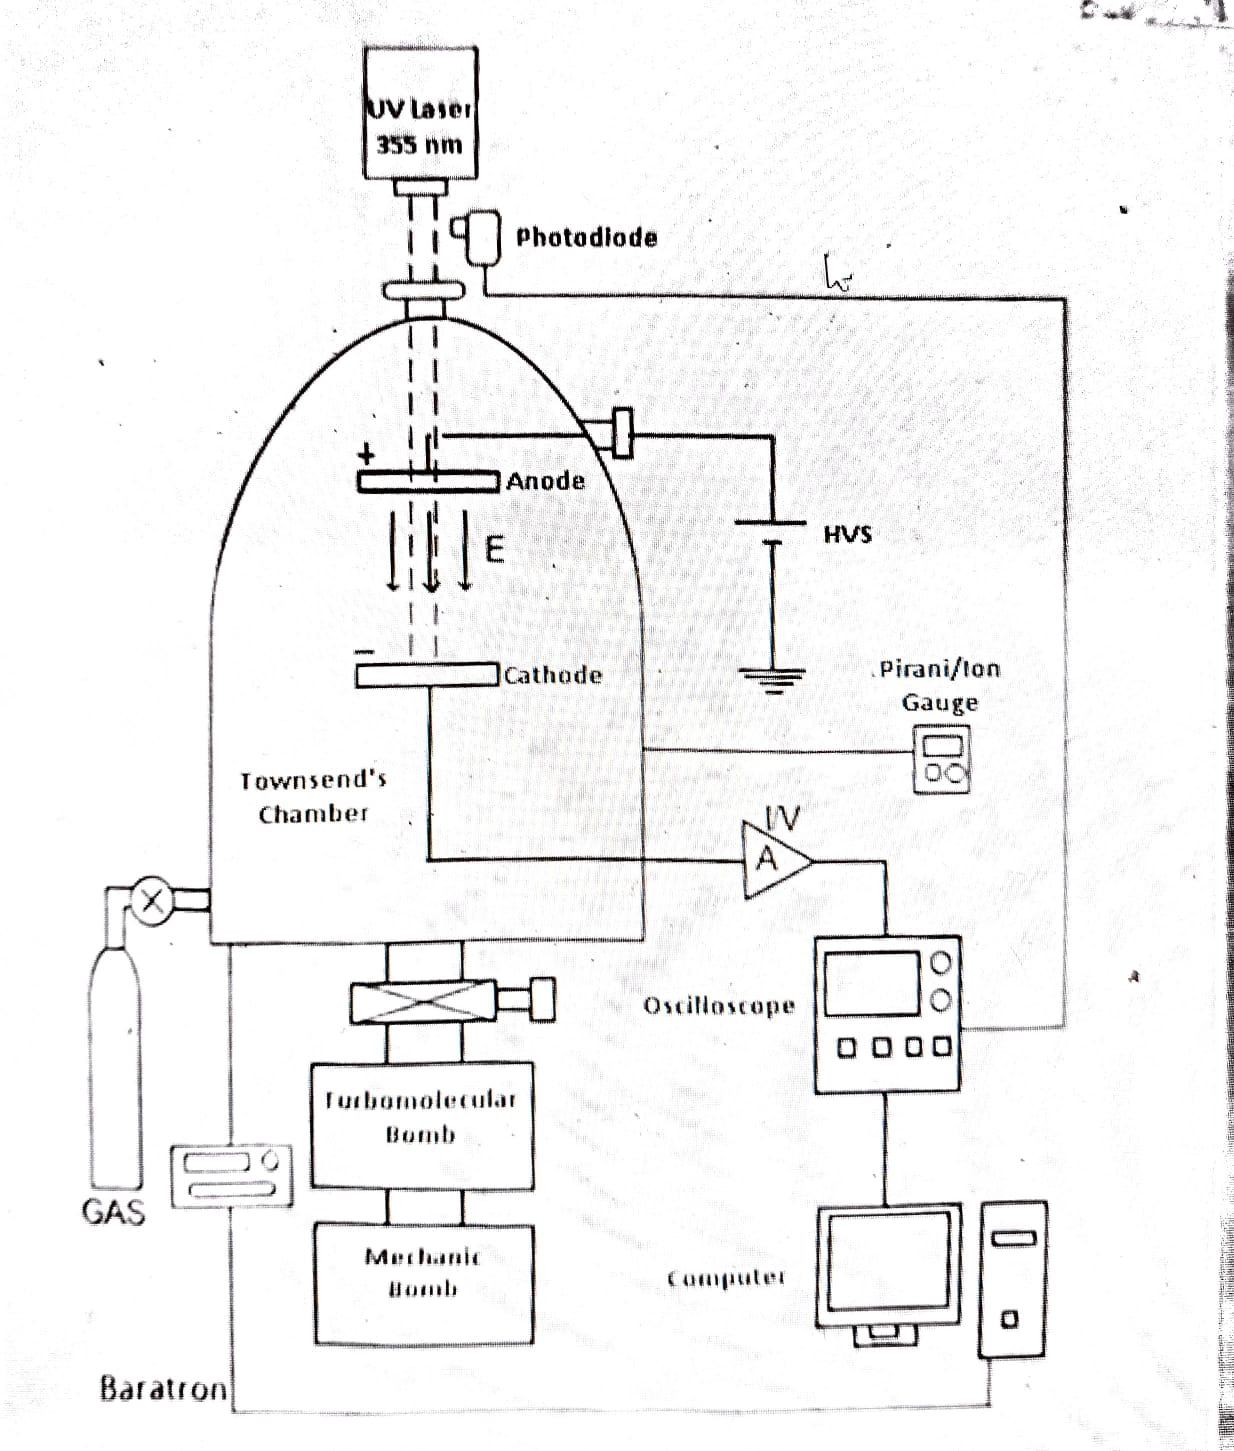
\includegraphics[scale=0.14]{figs/DiagramaTownsend.jpeg}
	\caption{Diagrama del arreglo experimental}
	\label{DiagT}
\end{figure}

En el computador modificamos la intensidad del láser y el voltaje suministrado. Comenzamos con 200 Torr...
\noindent 

\subsection{PARTE 2}
\noindent Se utilizó un módulo pre-fabricado para polarizar adecuadamente los electrodos de un bulbo 2D21 (Figura \ref{Diag1}). Se utilizaron dos fuentes de alimentación UNI-T UDP6721 para polarizar al filamento y para la polarización del ánodo-cátodo; para la primera se configuró una fuente a $2\,A$ y para la segunda a $1\,A$. Se siguió el diagrama de conexión de la Figura \ref{Diag2}, utilizando también dos multímetros Steren UNI-T MUL-600.

\begin{figure}[H]
	\centering
	
\includegraphics[scale=0.4]{figs/Diag1.png}
	\caption{Diagrama de conexión interna del módulo con el bulbo 2D21.}
	\label{Diag1}
\end{figure}

\begin{figure}%[H]
	\centering
	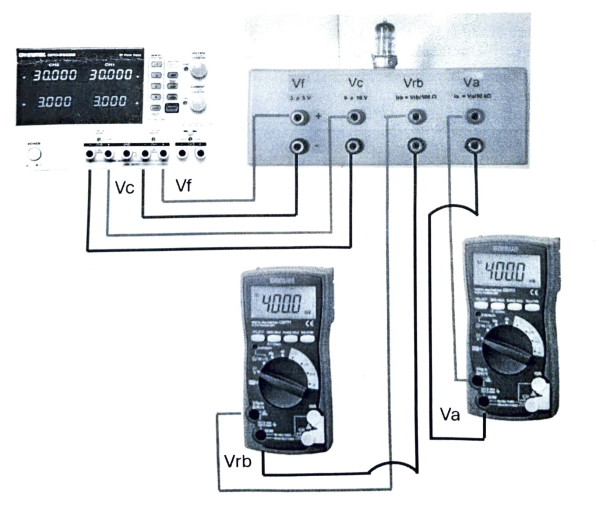
\includegraphics[scale=0.4]{figs/Diag2.png}
	\caption{Diagrama de conexión interna del módulo con el bulbo 2D21.}
	\label{Diag2}
\end{figure}

Una vez hecha las conexiones se incrementó el voltaje del filamento ($V_f$) hasta $2\,V$ y se dejó reposar durante $2$ minutos para que el filamento se calentara. Después, se varió el voltaje del cátodo ($V_c$) de $0\,V$ a $4\,V$ en pasos de $0.1\,V$ , y se tomó registro del voltaje del ánodo ($V_a$) y de la rejilla-bilndaje ($V_{rb}$) a través de los multímetros. Este procedimiento se repitió para un $V_f$ de $3\,V$ y $4\,V$, y se graficaron tanto $V_{rb} \textit{ vs. } V_c$ como $V_a \textit{ vs. } V_c$ para cada uno de los tres $V_f$.

Finamelmente, se hizo prueba de un software del laboratorio que automatiza el procedimiento anterior para un $V_f$ que nosotros le indiquemos, y el producto que devuelve es el registro de los voltajes $V_a$ y $V_{rb}$; así, también se hizo una comparación de los métodos de medición.